\documentclass{beamer}
\usepackage{amsmath}
\usepackage{amssymb}
\usepackage{amsfonts}
\usepackage[utf8]{inputenc}
\usepackage{graphics}
\usepackage{hyperref}
\usepackage{xcolor}
\usepackage{wasysym}
\usepackage{listings}
\usepackage{tikz}
\usepackage[normalem]{ulem}
\usepackage{textcomp}
\usepackage{verbatim}
\usepackage[T1]{fontenc}
\usepackage{lmodern}
\usepackage[framemethod=tikz]{mdframed}
\usetikzlibrary{shapes.callouts,shadows, calc}

\tikzset{note/.style={rectangle callout, rounded corners,fill=gray!20,drop shadow,font=\footnotesize}}    
\newcommand{\tikzmark}[1]{\tikz[overlay,remember picture] \node (#1) {};}    

\newcounter{image}
\setcounter{image}{1}

\makeatletter
\newenvironment{btHighlight}[1][]
{\begingroup\tikzset{bt@Highlight@par/.style={#1}}\begin{lrbox}{\@tempboxa}}
{\end{lrbox}\bt@HL@box[bt@Highlight@par]{\@tempboxa}\endgroup}

\newcommand\btHL[1][]{%
  \begin{btHighlight}[#1]\bgroup\aftergroup\bt@HL@endenv%
}
\def\bt@HL@endenv{%
  \end{btHighlight}%   
  \egroup
}
\newcommand{\bt@HL@box}[2][]{%
  \tikz[#1]{%
    \pgfpathrectangle{\pgfpoint{0pt}{0pt}}{\pgfpoint{\wd #2}{\ht #2}}%
    \pgfusepath{use as bounding box}%
    \node[anchor=base west,rounded corners, fill=green!30,outer sep=0pt,inner xsep=0.2em, inner ysep=0.1em,  #1](a\theimage){\usebox{#2}};
  }%
 \stepcounter{image}
}
\makeatother

\usetheme{Warsaw}
\usecolortheme{lily}
\setbeamercovered{transparent}
\setbeamertemplate{headline}{
  \begin{beamercolorbox}{section in head/foot}
    \vskip2pt\insertnavigation{\paperwidth}\vskip2pt
  \end{beamercolorbox}
}

\setbeamertemplate{footline}{
}

\author{
  {\tiny Tony Morris\\}
}

\xdefinecolor{darkgreen}{rgb}{0,0.35,0}
\lstset{
  tabsize=2,
  basicstyle=\ttfamily,
  moredelim=**[is][\btHL]{`}{`}
}
\lstdefinelanguage{java}{
  morekeywords={abstract,assert,boolean,break%
    byte,case,catch,char,class,const,continue%
    default,do,double,else,enum,extends,false%
    final,finally,float,for,goto,if,implements%
    import,instanceof,int,interface,long,native%
    new,null,package,private,protected,public%
    return,short,static,strictfp,super,switch%
    synchronized,this,throw,throws,transient%
    true,try,void,volatile,while},
  otherkeywords={=,=>,<-,<\%,<:,>:,\#,@},
  sensitive=true,
  morecomment=[l]{//},
  morecomment=[n]{/*}{*/},
  morestring=[b]",
  morestring=[b]',
  morestring=[b]"""
}
\lstdefinelanguage{csharp}
{
  sensitive=true,
  morekeywords=[1]{
  abstract, as, base, break, case,
  catch, checked, class, const, continue,
  default, delegate, do, else, enum,
  event, explicit, extern, false,
  finally, fixed, for, foreach, goto, if,
  implicit, in, interface, internal, is,
  lock, namespace, new, null, operator,
  out, override, params, private,
  protected, public, readonly, ref,
  return, sealed, sizeof, stackalloc,
  static, struct, switch, this, throw,
  true, try, typeof, unchecked, unsafe,
  using, virtual, volatile, while, bool,
  byte, char, decimal, double, float,
  int, lock, object, sbyte, short, string,
  uint, ulong, ushort, void},
  morecomment=[l]{//},
  morecomment=[s]{/*}{*/},
  morecomment=[l][keywordstyle4]{\#},
  morestring=[b]",
  morestring=[b]',
}
\lstdefinelanguage{haskell}{
  morekeywords={class,instance,where,do,data,newtype,default,deriving,module},
  otherkeywords={<-},
  sensitive=true,
  morecomment=[l]{--},
  morecomment=[n]{\{-}{-\}}, 
  morestring=[b]",
  morestring=[b]',
  morestring=[b]"""
}
\lstdefinelanguage{python}{
 keywords={catch, def, float, lambda, in, int, null, self, str, switch, typeof},
 keywordstyle=\color{ForestGreen}\bfseries,
 ndkeywords={boolean, throw, import},
 ndkeywords={return, class, if ,elif, endif, while, do, else, True, False , catch, def},
 ndkeywordstyle=\color{red}\bfseries,
 identifierstyle=\color{black},
 sensitive=false,
 comment=[l]{\#},
 morecomment=[s]{/*}{*/},
 commentstyle=\color{purple}\ttfamily,
 stringstyle=\color{red}\ttfamily,
}
\lstdefinelanguage{scala}{
  morekeywords={abstract,case,catch,class,def,%
    do,else,extends,false,final,finally,%
    for,forSome,if,implicit,import,lazy,match,%
    new,null,object,override,package,%
    private,protected,requires,return,sealed,%
    super,this,throw,trait,true,try,%
    type,val,var,while,with,yield},
  otherkeywords={=,=>,<-,<\%,<:,>:,\#,@},
  sensitive=true,
  morecomment=[l]{//},
  morecomment=[n]{/*}{*/},
  morestring=[b]",
  morestring=[b]',
  morestring=[b]"""
}
\lstdefinestyle{haskell}{
  language=haskell,
  basicstyle=\footnotesize\ttfamily,
  stringstyle=\color{darkgreen}\ttfamily,
  commentstyle=\color{gray}\ttfamily,
  keywordstyle=\footnotesize\color{blue}\ttfamily,
  tabsize=2,
  moredelim=**[is][\btHL]{`}{`}
}
\lstdefinestyle{java}{
  language=java,
  basicstyle=\footnotesize\ttfamily,
  stringstyle=\color{darkgreen}\ttfamily,
  commentstyle=\color{gray}\ttfamily,
  keywordstyle=\footnotesize\color{blue}\ttfamily,
  tabsize=2,
  moredelim=**[is][\btHL]{`}{`}
}
\lstdefinestyle{python}{
  language=python,
  basicstyle=\footnotesize\ttfamily,
  stringstyle=\color{darkgreen}\ttfamily,
  commentstyle=\color{gray}\ttfamily,
  keywordstyle=\footnotesize\color{blue}\ttfamily,
  tabsize=2,
  moredelim=**[is][\btHL]{`}{`}
}
\lstdefinestyle{csharp}{
  language=csharp,
  basicstyle=\tiny\ttfamily,
  stringstyle=\color{darkgreen}\ttfamily,
  commentstyle=\color{gray}\ttfamily,
  keywordstyle=\tiny\color{blue}\ttfamily,
  tabsize=2,
  moredelim=**[is][\btHL]{`}{`}
}
\lstdefinestyle{scala}{
  language=scala,
  basicstyle=\footnotesize\ttfamily,
  stringstyle=\color{darkgreen}\ttfamily,
  commentstyle=\color{gray}\ttfamily,
  keywordstyle=\footnotesize\color{blue}\ttfamily,
  tabsize=2,
  moredelim=**[is][\btHL]{`}{`}
}
% #866eaa
\definecolor{nicta-purple}{rgb}{0.5234,0.4297,0.6640}

\defbeamertemplate*{title page}{customized}[1][] {
  \centering
  \color{nicta-purple}
  \usebeamerfont{title}\inserttitle\par
  \bigskip
  \usebeamerfont{subtitle}\insertsubtitle\par
  \bigskip
  \bigskip
  \bigskip
  \bigskip
  \usebeamerfont{institute}\insertinstitute\par
  \bigskip
  \usebeamerfont{author}\insertauthor\par
  % \usebeamerfont{date}\insertdate\par
  \usebeamercolor[fg]{titlegraphic}\inserttitlegraphic
}

\logo{
\includegraphics[height=0.8cm]{image/data61-csiro.jpg}}


\setbeamercovered{transparent}

\begin{document}

\newmdenv[tikzsetting={draw=black,fill=white,fill opacity=0.7, line width=4pt},backgroundcolor=none,leftmargin=0,rightmargin=0,innertopmargin=4pt]{Conference}

\newmdenv[tikzsetting={draw=black,fill=white,fill opacity=0.7, line width=4pt},backgroundcolor=none,leftmargin=0,rightmargin=0,innertopmargin=4pt,skipbelow=\baselineskip,%
skipabove=\baselineskip]{TitleBox}

\title{\large Functional Programming in Aviation}
\institute[NICTA]{Data61, CSIRO}

{
  \usebackgroundtemplate{
\includegraphics[width=1.0\paperwidth]{image/title-background.png}}

  \begin{frame}[plain] 

  \begin{TitleBox}
    \begin{center}
    {\huge \inserttitle}

    \hspace{1em}
    
    {\huge \insertsubtitle}
    \end{center}
  \end{TitleBox}

  \vspace{3em}

  \begin{Conference}
    \begin{center}
    \tiny{devtalk, January 2017}

    \hspace{1em}

    {\insertauthor}
    \end{center}
  \end{Conference}

  \end{frame}
}

\begin{frame}
\begin{center}
Why aviation?
\end{center}
\end{frame}

\begin{frame}
\frametitle{Aviation}
\begin{block}{I live near here}
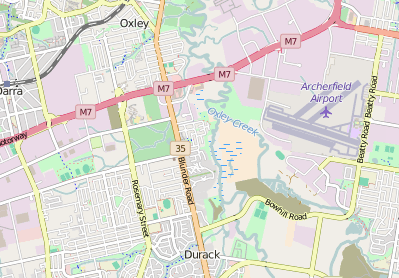
\includegraphics[height=0.5\textheight]{image/archerfield-map.png}
\end{block}
\end{frame}

\begin{frame}
\frametitle{Aviation}
\begin{block}{This is the 10L/28R circuit pattern for Archerfield (YBAF)}
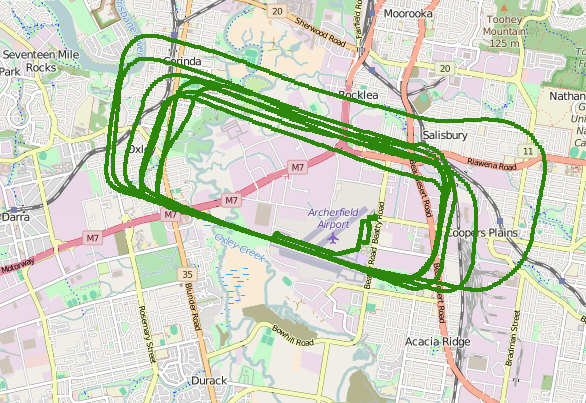
\includegraphics[height=0.5\textheight]{image/archerfield-circuit.png}
\end{block}
\end{frame}

\begin{frame}
\frametitle{Aviation}
\begin{block}{and I'd see this on my way home}

\includegraphics[height=0.5\textheight]{image/aeroplane-approach.jpg}
\end{block}
\end{frame}

\begin{frame}
\frametitle{Aviation}
\begin{block}{This is me on my way home}

\includegraphics[height=0.5\textheight]{image/aeroplane-graze-photographer.jpg}
\end{block}
\end{frame}

\begin{frame}
\frametitle{Aviation}
\begin{block}{and so}

\includegraphics[height=0.5\textheight]{image/thought-bubble-thats-it.png}
\end{block}
\end{frame}

\begin{frame}
\frametitle{Aviation}
\begin{block}{In November 2015, I did this}

\includegraphics[height=0.5\textheight]{image/flight-school-google.png}
\end{block}
\end{frame}

\begin{frame}
\frametitle{A domestic argument ensued}
\begin{block}{My lovely wife Amanda was like}

\includegraphics[height=0.5\textheight]{image/thought-bubble-dollars.png}
\end{block}
\end{frame}

\begin{frame}
\frametitle{A compromise was reached}
\begin{block}{and I was like}

\includegraphics[height=0.3\textheight]{image/tom-cruise.png}
\end{block}
\end{frame}

\begin{frame}
\frametitle{The argument was over}
\begin{block}{and Amanda was like}

\includegraphics[height=0.5\textheight]{image/thought-bubble-good-point.png}
\end{block}
\end{frame}

\begin{frame}
\frametitle{Pilot Licences}
\begin{block}{There are (loosely) four levels of CASA pilot licence}
\begin{enumerate}
\item RPL
  \begin{itemize}
  \item \tiny{MTOW <= 1500kg}
  \item \tiny{no navigation beyond 25nm (46km) from departure point}
  \item \tiny{day time, VFR only}
  \item \tiny{class 1 or 2 aviation medical for >1 PAX}
  \end{itemize}
\item PPL
  \begin{itemize}
  \item \tiny{MTOW <= 5700kg}
  \item \tiny{can navigate}
  \item \tiny{no commercial ops}
  \item \tiny{day time, VFR only}
  \item \tiny{class 1 or 2 aviation medical for >1 PAX}
  \end{itemize}
\item CPL
  \begin{itemize}
  \item \tiny{commercial ops}
  \item \tiny{class 1 aviation medical}
  \end{itemize}
\item ATPL
  \begin{itemize}
  \item \tiny{>= 1500 hours for aeroplane category}
  \item \tiny{>= 1000 hours for helicopter category}
  \end{itemize}
\end{enumerate}
\end{block}
\end{frame}

\begin{frame}
\frametitle{Aviation}
\begin{block}{This is a story about some things I have learned about aviation and how we can
apply our programming tools to improve efficiency and safety.}
\begin{itemize}
\item \tiny{legislation, regulation, services}
\item \tiny{pilot logbooks}
\item \tiny{aeronautical navigation}
%  include AvPlan and FAA failed georectification
% reasons why georectification is even a thing
%  NZ incident
\item \tiny{calculating aircraft weight and balance}
\item \tiny{ADS-B, aircraft transmitting parameters to other aircraft and ground stations, denoting a current status}
\end{itemize}
\end{block}
\end{frame}


\end{document}
